\chapter{Percussion pattern transcription and discovery}\label{chap:percpatt}
\begin{epigraphs}
  \qitem{The metaphorical usage of `language' for a musical system is paralleled by a literal usage that refers to the ways in which many drum musics may be represented with spoken syllables.}{\citeA{kippen:89:perclanguage}}
\end{epigraphs}
%\textit{Chapter in brief: Present the second thesis problem of percussion pattern discovery. This chapter presents preliminary work in percussion pattern transcription as applied to both CM and HM, with a special emphasis on methodology but less so on results. Beijing Opera is used as a -test case before applying on CM and HM. The chapter is short and shallow - include mainly for completeness. The material comes from ICASSP 2014, ISMIR 2014, ISMIR 2015 papers and unpublished results so far.}
% \update{TODO: Intro to be cleaned up}
\noindent Percussion plays an important role in Indian art music with a significant freedom to improvise, leading a wide variety of percussion patterns that help to create multiple layers of rhythm. An analysis of these percussion patterns hence is an important step towards developing rhythm similarity measures. We wish to discover percussion patterns from audio recordings in a data-driven way, while using a musically meaningful representation for percussion patterns. 

We address the task of percussion pattern \index{Percussion pattern}discovery in this chapter taking an approach of transcription followed by a search for patterns. The work presented in the chapter is basic and exploratory, and only for demonstrating the utility of a syllabic percussion system in percussion pattern transcription and discovery. Most experiments presented contain preliminary results, needing further work. The goals of the chapter are: 
\begin{enumerate}[leftmargin=*]
 \item To discuss two broad approaches to percussion transcription. To focus on timbre based transcription, and to present how meaningful representations can be obtained for overall timbres of percussion strokes in syllabic percussion systems.
 \item To present an approach to percussion pattern transcription and discovery in syllabic percussion systems based on a speech recognition framework.
 \item To present experiments on \gls{jingju} percussion patterns, as a simpler example test case of percussion pattern transcription and pattern classification. To extend the approach to Indian art music, and evaluate it on mridangam and tabla solo datasets. 
 \item To identify the advantages and shortcomings of such an approach, with possible future research directions to pursue. 
\end{enumerate}
We first start by describing two broad approaches that can be taken for the task of percussion pattern transcription. 
%
\section{Approaches} %  to percussion pattern transcription and discovery
% \note{Two approaches - onset detection + instrument ID, or combined. But this does not make use of the syllabic structure, and hence we have the new method based on speech recognition.}
Percussion transcription aims to transcribe an audio recording of a percussion solo into a time aligned sequence of symbols. Depending on the symbol set chosen and the acoustic events being modeled, transcription can be approached in two different broad ways. The two approaches differ mainly in the way they define percussion patterns in audio. % and transcribe and discover 
\subsubsection{Transcription based on individual instruments}
An audio recording can be transcribed into time aligned sequence of individual percussion instrument stroke onsets, e.g. transcribing a drum solo into a sequence of bass, hi-hats and snare drum onsets. The output of such a task is a drum score showing all the drums, and their onset times. A percussion pattern can then be described and represented using that score, using the onset information from all instruments. Such an approach is useful for transcription from drum mixtures, when percussion patterns are defined as a sequential combination of different instruments, each retaining their own musical identity. Since most percussion solos have simultaneous strokes from multiple instruments, such an approach needs a decomposition of the audio containing drum mixtures into individual drum components. As a pre-processing step, an instrument-wise onset detection might be needed. 

As discussed before in \secref{sec:bkgnd:sotapercpatt}, event-based transcription algorithms~\cite{gillet:04:drumloops,gouyon:02:pulse,goto:94:soundSep,gillet:08:transcription} segment the input signal based on percussion events then extract and classify features from these segments to uncover its musically meaningful content, such as onsets. Source separation based methods~\cite{paulus:05:drum,smaragdis:04:convNMF,abdallah:03:probability} decompose the input audio signal containing drum mixtures into basis functions capturing spectral characteristics of the sources (ideally, individual percussion instruments). \citeA{tian:14:icassp} present an exploratory study on the use of \gls{NMF} based source separation techniques for instrument specific onset detection in \gls{jingju} percussion instrument ensembles, aiming at providing a baseline for further research in \gls{jingju} percussion transcription. 
%
\subsubsection{Transcription based on overall timbre}
A contrasting approach is to consider the overall timbre sequence of a percussion solo, without any regard to individual instruments. A percussion pattern is then defined as a sequence of combined instrument timbres and the goal is to transcribe an audio recording into a sequence of such combined timbres. Such an approach is useful when percussion patterns can be defined based on timbral sequences e.g. in syllabic percussion systems. A notable limitation of the approach however is when a pattern cannot be accurately defined by the overall timbre, and individual instrument timbres are necessary, as often is the case with a drum set. 

In syllabic percussion\index{Syllabic percussion} systems, patterns can be defined using syllables, which is both musically meaningful and accurate in representation. In certain percussion systems such as in \gls{jingju} percussion, the syllables represent the overall combined timbre of a percussion ensemble, while in Indian art music (both Carnatic and Hindustani music), the syllables represent the different timbres that can be produced by the (often) single percussion instrument used, either the \gls{tabla} or the mridangam. In either case, the overall timbre represented by the syllable is sufficient to define a percussion pattern. In such a case, a percussion pattern can be represented solely based on these syllables and transcribed as such. 

In this chapter, we explore only the second approach, using syllables to define overall timbres of percussion strokes. We then use them to define, transcribe and discover percussion patterns. In the remainder of the chapter, the goal is to test the effectiveness and relevance of percussion syllables in representation and modeling of percussion patterns for automatic transcription and discovery. Since these syllables have a clear analogy to speech and language, the transcription task has a definite analogy to speech recognition and we can apply several tools and knowledge from this well explored research area with many state of the art algorithms and systems~\cite{huang:10:sroverview}. 

The final goal is to automatically discover percussion patterns from segmented percussion solo audio recordings of Indian art music, and we take a transcription + search approach as briefly discussed in \secref{sec:probdef:thesispattern}. The task however is challenging since it requires a concrete definition of a percussion pattern, while such a definition of what constitutes a percussion pattern is ambiguous in Indian art music. Further, Indian percussion has a great scope for improvisation within the framework of the \gls{tala}. This leads a large number of percussion patterns that can be played on the mridangam and tabla, which makes it further difficult to define relevant percussion patterns without ambiguity. We address this issue by making the discovery unsupervised and data-driven, by using transcribed ground truth music scores to define relevant patterns. 

Given the complexity of the task in Indian art music due to ill-defined large number of patterns, we consider the case of percussion patterns in \gls{jingju} as an initial test case for our hypothesis and methods. Percussion patterns in \gls{jingju} are simpler in both these aspects when compared to Indian art music: \gls{jingju} percussion patterns are well defined and limited in number. Once we demonstrate and validate our hypothesis with \gls{jingju}, we extend the methodology to Indian art music, with a data-driven but extendable definition of a percussion pattern. Since there are a limited number of \gls{jingju} percussion patterns, the problem of pattern discovery in \gls{jingju} is simplified into a pattern classification task, as is described further in the following section. 
%
\section[The case of Beijing opera]{The case of Beijing opera (\Gls{jingju})}\label{sec:ppclassify:jingju}
\begin{figure}
\captionsetup[subfigure]{labelformat=empty}
\centering
\subfloat[]{\label{fig:boperc:instwav} \includegraphics[width=0.95\textwidth]{jingjuPatts/jingju-stroke-waveform.pdf}}\\ \vspace{-1cm} 
\subfloat[]{\label{fig:boperc:instspec} \hspace{1.2mm} \includegraphics[width=0.93\textwidth]{jingjuPatts/jingju-stroke-spectrum.pdf}} 
\caption[Waveform and spectrogram of \gls{jingju} percussion strokes]{The waveform and spectrogram of an audio example containing all four instrument groups of \gls{jingju}. The top panel shows the waveform and the bottom panel is the spectrogram, the x-axis for both panels is time (in seconds). The vertical lines (in red) mark the onsets of the instruments. The onsets are labeled to indicate the specific instruments: \gls{bangu}-1, \gls{daluo}-2, \gls{naobo}-3, \gls{xiaoluo}-4.}\label{fig:bo:instwavspec}
\end{figure}
To recall from \secref{sec:bkgnd:bopercussion}, percussion ensemble in \gls{jingju} consists of five instruments played by four musicians, and can be grouped based on timbre into four instrument groups - \gls{bangu} (clapper-drum), \gls{xiaoluo} (small gong), \gls{daluo} (big gong) and \gls{naobo} (cymbals). The waveform and spectrogram of an audio example with all four of these instrument classes is shown in \figref{fig:bo:instwavspec}\footnote{The audio example is available here: \url{http://www.freesound.org/people/ajaysm/sounds/205971/}}. We can see the amplitude dynamics and spectral shapes for each instrument. \Gls{daluo} has a falling pitch, while \gls{xiaoluo} has a rising pitch profile. \Gls{naobo} has a broadband spectrum with significant energy in higher frequencies, as is characteristic of cymbals. Onsets generated by \gls{bangu} are sharp, have a much lower amplitude and shorter transient time, and happen in higher density than those generated by the other instruments. Hence, the \gls{bangu} onsets are easily masked by the cymbals and gongs. We can also see how the \gls{bangu} stroke is masked by an adjoining \gls{xiaoluo} stroke (0-0.5s in \figref{fig:bo:instwavspec}).

Using combinations of these instruments, several different combined percussion strokes are produced, each of which is labeled with an onomatopoeic oral mnemonic syllable\index{Oral mnemonic syllable}. Since there are many syllables that map to a single timbre, we reduced the complete set of syllables into five syllable groups - \syl{DA}, \syl{TAI}, \syl{QI}, \syl{QIE}, and \syl{CANG}, as listed in \tabref{tab:bo:sylmap}. The use of these oral syllabic sequences simplify and unify the representation of these patterns played by an ensemble. 

To further recall \secref{sec:bkgnd:bopercussion}, the percussion patterns in \gls{jingju} music are sequences of strokes played by different combinations of the percussion instruments, and the resulting variety of timbres are transmitted using oral syllables as mnemonics. Each percussion pattern is a sequence of syllables in their pre-established order, along with their specific rhythmic structure and dynamic features. Each particular pattern has a single unique syllabic representation shared by all the performers. Hence, the use of these oral syllabic sequences simplify and unify the representation of these patterns played by an ensemble, making them optimal for the transcription and automatic classification of the patterns.
\begin{figure}
\captionsetup[subfigure]{labelformat=empty}
\centering
\subfloat[]{\label{bowaveform} \includegraphics[scale=0.4]{percPatterns/waveform-shanchui.pdf}}\\ \vspace{-1cm}
\subfloat[]{\label{bospectrum} \hspace{-0.9mm} \includegraphics[scale=0.4]{percPatterns/spectrum-shanchui.pdf}}
\caption[Waveform and spectrogram of the pattern \gls{shanchui}]{The waveform and spectrogram of an audio example of the pattern \gls{shanchui}. The top panel shows the waveform and the bottom panel is the spectrogram. The vertical lines (in red) mark the onsets of the syllables. The onsets are labeled to indicate the specific syllable group: \syl{DA}-1, \syl{TAI}-2, \syl{QI}-3, \syl{QIE}-4, and \syl{CANG}-5 (\syl{QI} is not present in this pattern). The score for the pattern is shown in \protect\figref{fig:bopatt:shanchui}. Notice that the audio example has two additional repetitions of the sub-sequence \syl{CANG}-\syl{TAI}-\syl{QIE}-\syl{TAI} in the pattern.}\label{fig:bopercpatt:audio}
\end{figure}

A performance starts and ends with percussion patterns, they generally introduce and conclude arias, and mark transition points within them. The patterns accompany the actors' movements on stage and set the mood of the play, the scene, the aria or a section of the aria. An automatic description of these percussion patterns is thus quite important in providing the overall description of the aria. Therefore, the detection and characterization of percussion patterns is a fundamental task for the description of the music dimension in Beijing opera. In practice, there is a limited set of named patterns that are played in performance. 

Though the patterns are limited in number and predefined, there are several challenges to the problem of percussion pattern transcription and classification. Being an oral tradition, the syllables used for the representation of the patterns lack full consistency and general agreement. The result being that one particular timbre might be represented by more than one syllable. Furthermore, the syllabic representation conveys information for the conjoint timbre of the ensemble, so only the main structural sounds are represented. In an actual performance, a particular syllable might be performed by different combinations of instruments - e.g. in \figref{fig:bopatt:shanchui}, the first occurrence of the syllable \syl{TAI} is played just by the \gls{xiaoluo}, but in the rest of the pattern is played by \gls{xiaoluo} and the \gls{bangu} together. In fact, generally speaking, the strokes of the \gls{bangu} are seldom conveyed in the syllabic sequence (as can be seen in the third measure in \figref{fig:bopatt:shanchui} for the second sixteenth-note of the \gls{bangu}), except for the introductions and other structural points played by the drum alone. As indicated in \tabref{tab:bo:sylmap}, \syl{CANG} is mostly a combination of all the three metallophones, but in some cases, \syl{CANG} can be played with just the \gls{daluo}, or just the \gls{daluo}+\gls{naobo} combination. 

In the cases where the percussion pattern is to accompany the movements of actors on stage, certain syllable subsequences in the pattern are repeated indefinitely. This causes the same pattern in different performances to have variable lengths, and these repetitions need to be explicitly handled. The timing of these patterns is expressive and matches the acting in the scene, and hence we consider only the sequence of syllables and do not consider timing relationships between the syllables to define patterns. Finally, although the patterns are usually played in isolation, in many cases the string instruments or even the vocals can start playing before the patterns end, presenting challenges in identification and classification. \figref{fig:bopercpatt:audio} shows an audio example of the pattern \gls{shanchui}, along with time aligned markers to indicate the syllable onsets. The spectrogram also shows the timbral characteristics of the percussion instruments \gls{xiaoluo} (increasing pitch) and \gls{daluo} (decreasing pitch). Some variation to the notated score can also be seen, such as expressive timing and additional insertion of syllables.

At the outset, it is clear that Beijing opera percussion patterns are well defined and limited in number. Further, in \gls{jingju}, the recognition of the pattern as a whole is more important than an accurate syllabic transcription of the pattern. Due to the limited set of pattern classes and owing to all the variations possible in a pattern, we are primarily interested in classifying an audio pattern into one of the possible pattern classes. Syllabic transcription is only considered as an intermediate step towards pattern classification. The named patterns can be used to build a library of patterns. The patterns can be referred to as ``pattern classes" for the purpose of classification, and classifying an instance of a pattern occurring in the audio recording of an aria into one of these pattern classes is thus a primary task. 
% 
\subsection{Percussion pattern classification}
Beijing opera percussion pattern transcription and classification is a first test case for percussion pattern discovery approaches. In this work, we restrict to five predominantly used percussion patterns in \gls{jingju} - \gls{daobantou}, \gls{manchangchui}, \gls{duotou}, \gls{xiaoduotou}, and \gls{shanchui} (pattern scores provided in \figref{fig:bopatt:scores}). Further, we restrict ourselves to percussion patterns that occur at the introduction of the aria, since they convey significant information about the structure of the aria that follows it, e.g. \gls{daobantou} pattern is followed by an aria in \gls{banshi} \gls{daoban}. %\comment{Check with Rafa, XX}  

We now present a formulation for transcription and recognition of syllable based audio percussion patterns, and evaluate it on the \acrfull{BOPP} (see \secref{sec:dataset:bopp}). The dataset is a collection of 133 audio percussion patterns spanning five different pattern classes, with over 2200 syllables in total. There is a significant analogy of this task to connected word speech recognition using word models. Syllables are analogous to words and a percussion pattern to a sentence - a sequence of words. There are language rules to form a sentence using a vocabulary, just as each percussion pattern is formed with a defined sequence of syllables from a vocabulary. However unlike in the case of speech recognition where infinitely many sentences are possible, in our case we have a small number of percussion patterns to be recognized.

Similar to the work by \citeA{nakano:04:voicePerc}, we explore a speech recognition based framework in this study. Their approach is different from ours in the sense that the onomatopoeic representations they used were created by the authors, while we are relying on already existing oral traditions. To the best of our knowledge, \citeA{ajay:14:ismirbo} presented the first work that explored automatic transcription and classification of syllable based percussion patterns, as applied to Beijing opera. The method and results presented in this section are from that work. 

Following the notation presented in \secref{sec:probdef:thesispattern}, consider a set of $\nPercPatterns$ pattern classes $\pattSet = \{\percPattSeq_1, \percPattSeq_2, \cdots \percPattSeq_\nPercPatterns\}$, each of which is a sequence of syllables from the set of syllables $\sylSet = \{\sylSetVar_1, \sylSetVar_2, \cdots \sylSetVar_\nSyllables\}$, where $\nSyllables$ is the total number of syllables in the set. Hence, a percussion pattern is represented as $\percPattSeq_i = [\sylVar_1, \sylVar_2, \cdots, \sylVar_{\pattLen_i}]$ where $\sylVar_j \in \sylSet$ and $\pattLen_i$ is the length of $\percPattSeq_i$. Given a test audio signal $\signal$ containing a percussion pattern, the transcription task aims to obtain a syllable sequence $\percPattSeq^{\optstar} = [\sylVar_1, \sylVar_2, \cdots, \sylVar_{\pattLen^{\optstar}}]$ and the classification task aims to assign $\percPattSeq^{\optstar}$ into one of the patterns in the set $\pattSet$. 

The syllables are non-stationary signals and to model their timbral dynamics, we build an \gls{HMM} for each syllable (analogous to a word-\gls{HMM}). Using these syllable \glspl{HMM} and a language model, an input audio pattern is transcribed into a sequence of syllables using Viterbi decoding\index{Viterbi decoding}, and then classified to a pattern class in the library using a measure of distance.
\begin{figure}[t]
\centering
 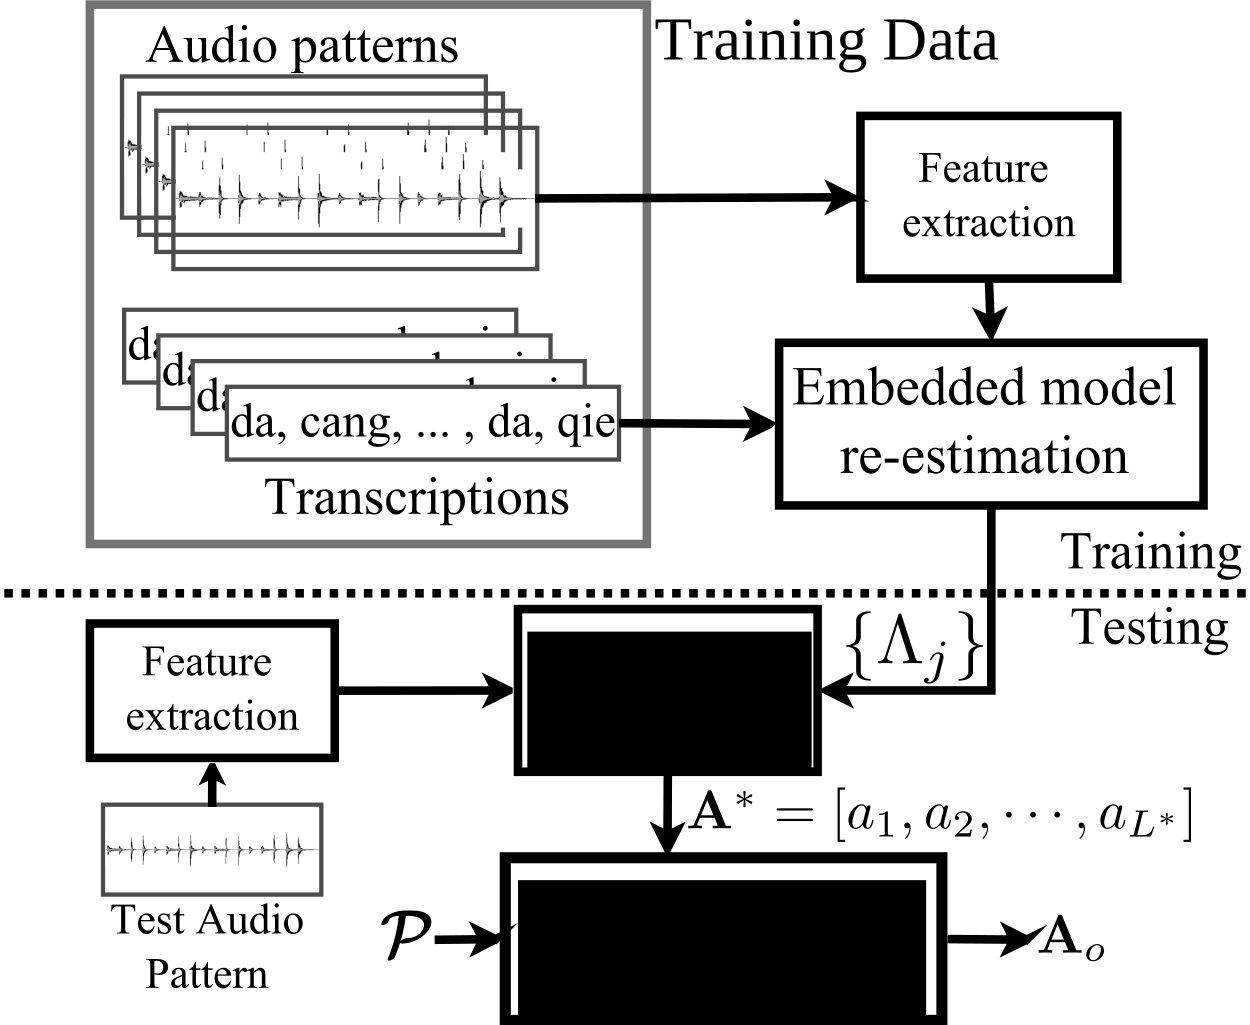
\includegraphics[width=\textwidth]{blockDiags/blockDiagJingjuPercClassify.pdf}
\caption[Block diagram: \Gls{jingju} percussion pattern classification]{The block diagram \gls{jingju} percussion pattern classification approach}\label{fig:BD:jingjuPercClassify}
\end{figure}

A block diagram of the approach is shown in \figref{fig:BD:jingjuPercClassify}. We first build syllable level \glspl{HMM} $\{\hmmSym_j\}$, $1 \leq j \leq \nSyllables (= 5)$, for each syllable $\sylSetVar_j$ using features extracted from the training audio patterns. We use the \gls{MFCC} features to model the timbre of the syllables. To capture the temporal dynamics of syllables, we add the velocity and the acceleration coefficients of the \gls{MFCC}. The stereo audio is converted to mono, since there is no additional information in stereo channels. The 13 dimensional (including the zeroth coefficient) \gls{MFCC} features are computed from audio patterns with a frame size of 23.2 ms and a shift of 5.8 ms. We also explore the use of energy (as measured by the zeroth \gls{MFCC} coefficient) in classification performance. Hence we have two sets of features, \acrshort{MFCCODA}, the 39 dimensional feature including the zeroth, delta (velocity) and double-delta (acceleration) coefficients, and \acrshort{MFCCDA}, the 36 dimensional vector without the zeroth coefficient. 

We model each syllable using a 5-state left-to-right \gls{HMM} including an entry and an exit non-emitting states. The emission densities for each state is modeled with a four component \gls{GMM} to capture the timbral variability in syllables. We experimented with eight and sixteen component \gls{GMM}, but with little performance improvement. Since we do not have time aligned transcriptions in the \acrshort{BOPP} dataset, an isolated \gls{HMM} training for each syllable is not possible. Hence we use an embedded model Baum-Welch re-estimation~\cite{huang:90:hmm} to train the \glspl{HMM} using just the syllable sequence corresponding to each feature sequence. The \glspl{HMM} are initialized with a flat start using all of the training data. All the experiments were done using the \acrfull{HTK} \cite{young:06:htkbook}. 

Given a test audio pattern, we use these syllable \glspl{HMM} to obtain a rough syllabic transcription and then classify the test pattern into one of the pattern classes in the library based on a measure of distance between the test pattern and the pattern classes. Since we only need a rough syllabic transcription independent of the pattern class, we treat the test audio pattern as a first order time-homogenous discrete Markov chain, which can consist of any finite length sequence of syllables, with uniform unigram and bigram (transition) probabilities, i.e. $P(\sylVar_1 = \sylSetVar_i) = 1/\nSyllables$ and $P(\sylVar_{k+1} = \sylSetVar_j \mid \sylVar_k = \sylSetVar_i) = 1/\nSyllables$, $ 1 \leq i,j \leq \nSyllables$, with $k$ being the sequence index. This also forms a simple uninformed language model\index{Language model} for forming the percussion patterns using syllables. Given a feature sequence extracted from test audio pattern, we use the \glspl{HMM} $\{\hmmSym_j\}$ to do a Viterbi (forced) alignment, which aims to provide the best sequence of syllables $\percPattSeq^{\optstar}$, given a syllable network constructed from the language model. 

Given the decoded syllable sequence $\percPattSeq^{\optstar}$, we compute the string edit distance \cite{navarro:01:strDist} between $\percPattSeq^{\optstar}$ and patterns in the set $\pattSet$. The use of edit distance is motivated by two factors. First, due to errors in Viterbi alignment, $\percPattSeq^{\optstar}$ can have insertions (\strInsErr), deletions (\strDelErr), substitutions (\strSubErr), and transposition (\strTrnErr) of syllables compared to the ground truth. Secondly, to handle the allowed variations in patterns, an edit distance is preferred over an exact match to the sequences in $\pattSet$. We explore the use of two different string edit distance measures, Levenshtein distance ($\distMeas_{1}$) that considers \strInsErr, \strDelErr, \strSubErr\ errors and the Damerau–Levenshtein distance ($\distMeas_2$) that considers \strInsErr, \strDelErr, \strSubErr, and also \strTrnErr\ errors~\cite{navarro:01:strDist}. 

As discussed earlier, there can be repetitions of a subsequence in some patterns. Though the number of repetitions is indefinite, we observed in the dataset that there are at most two repetitions in a majority of pattern instances. Hence for the pattern classes that allow repetition of a sub-sequence, we compute the edit distance for the cases of zero, one and two repetitions and then take the minimum distance obtained among the three cases. This way, we can handle repeated parts in a pattern. Finally, the $\percPattSeq^{\optstar}$ is assigned to the pattern class $\percPattSeq_o \in \pattSet$ for which the edit distance $\distMeas$ (either $\distMeas_1$ or $\distMeas_2$) is minimum, as in \eqnref{eqn:bo:pattclassify}.  
\begin{equation}
\percPattSeq_o = \underset{1 \leq j \leq \nPercPatterns}{\argmin}\;\distMeas(\percPattSeq^{\optstar},\percPattSeq_j) \label{eqn:bo:pattclassify}
\end{equation}
%
\subsection{Results and discussion}\label{sec:boperc:results}
We present the syllable transcription and pattern classification results on the \acrshort{BOPP} dataset described in \secref{sec:dataset:bopp}. The results shown in \tabref{tab:ppres:bopp} are the mean values in a leave-one-out cross validation. We report the syllable transcription performance using the measures of Correctness ($\corrMeas$) and Accuracy ($\accuMeas$). If $\pattLen$ is the length of the ground truth sequence, then the two measures are defined as,  
\begin{eqnarray}\label{eqn:pp:straccu}
\corrMeas & = & \frac{\pattLen - \strDelErr - \strSubErr}{\pattLen} \\
\accuMeas & = & \frac{\pattLen - \strDelErr - \strSubErr - \strInsErr}{\pattLen}
\end{eqnarray}
The Correctness measure penalizes deletions and substitutions, while Accuracy measure additionally penalizes insertions too. The pattern classification performance is shown for both edit distance measures $\distMeas_1$ and $\distMeas_2$ in \tabref{tab:ppres:bopp}. All the results are reported for both the features, \acrshort{MFCCODA} and \acrshort{MFCCDA}. The difference in performance between the two features was found to be statistically significant for both Correctness and Accuracy measures in a Mann-Whitney U test at $p = 0.05$, assuming an asymptotic normal distribution \cite{mann:47:Utest}.

In general, we see a good pattern classification performance despite a low syllable transcription accuracy. We see that the feature \acrshort{MFCCODA} leads to a better performance with syllable transcription, while both kinds of features provide a comparable performance for pattern classification. Though syllable transcription is not the primary task we focus on, an analysis of its performance provides several insights. The set of percussion instruments in Beijing opera is fixed, but there can be slight variations across different instruments of the same kind. The training examples are varied and representative, and models built can be presumed to be source independent. Nevertheless, there can be unrepresented syllable timbres in test data leading to a poorer transcription performance. A bigger training dataset can improve the performance in such a case. The energy (zeroth) co-efficient provides significant information about the kind of syllables and hence gives a better syllable transcription performance. 
\begin{table}
\centering
\begin{tabular}{@{}lcccccc@{}} \toprule
\multirow{2}{*}{Feature} & & \multicolumn{2}{c}{Syllable} & & \multicolumn{2}{c}{Pattern}\tabularnewline 
 & & $\corrMeas$ & $\accuMeas$ & & $\distMeas_1$ & $\distMeas_2$\tabularnewline \midrule
\acrshort{MFCCDA} & & 78.14 & 26.32 & & 93.23 & 89.47\tabularnewline 
\acrshort{MFCCODA} & & 84.98 & 39.63 & & 91.73 & 89.47\tabularnewline \bottomrule
\end{tabular}
\caption[Transcription and classification results on \acrshort{BOPP} dataset]{Syllable transcription and pattern classification performance on \acrshort{BOPP} dataset, with Correctness ($\corrMeas$) and Accuracy ($\accuMeas$) measures for syllable transcription. Pattern classification results are shown for both distance measures $\distMeas_1$ and $\distMeas_2$. All values are in percentage.} \label{tab:ppres:bopp}
\end{table}
%
\begin{table}
\centering
\begin{tabular}{@{}ll|cccccc@{}}\toprule
Pattern class & Total & ID & 1 & 2 & 3 & 4 & 5 \tabularnewline \midrule
\gls{daobantou} & 62 & 1 & 100 &  &  &  &  \tabularnewline 
\gls{manchangchui} & 33 & 2 & & 93.9 &  &  & 6.1 \tabularnewline 
\gls{duotou} & 19 & 3 &10.5 &  & 68.4 &  & 21.1 \tabularnewline 
\gls{xiaoduotou} & 11 & 4 & &  &  18.2 & 81.8 & \tabularnewline 
\gls{shanchui} & 8 & 5 & & 12.5 &  &  & 87.5 \tabularnewline \bottomrule
\end{tabular}
\caption[Confusion matrix for percussion pattern classification in \acrshort{BOPP} dataset]{The confusion matrix for pattern classification in \acrshort{BOPP} dataset, using the feature \acrshort{MFCCODA} with $\distMeas_1$ distance measure. The first and second column show the pattern class label and the total examples in each class, and class labels correspond to the ID in \tabref{tab:dataset:bopp}. The rows and column headers represent the True Class and Assigned Class, respectively. All other values are in percentage and the empty blocks are zeros (omitted for clarity).} \label{tab:ppres:boppconf}
\end{table}

We see that the Correctness is higher than Accuracy showing that the exact sequence of syllables, as indicated in the score was not achieved in a majority of the cases, with several insertion errors. This is due to the combined effect of errors in decoding and allowed variations in patterns. However, an edit distance based distance measure for classification is quite robust in the present five class problem and provides a good classification performance, despite the low transcription accuracy. 

Both distance measures provide comparable performance, indicating that the number of transposition errors are low. To see if there are any systematic classification errors, we compute a confusion matrix (\tabref{tab:ppres:boppconf}) with one of the well performing configurations: \acrshort{MFCCODA} with $\distMeas_1$ distance. We see that \gls{duotou} (ID = 3) has a low recall, and gets confused with \gls{shanchui} (ID = 5) often. A close examination of the scores showed that a part of the pattern duotou (\figref{fig:bopatt:duotou}) is contained within shanchui (\figref{fig:bopatt:shanchui}), which explains the source of confusion. From the scores, we also see that \gls{xiaoduotou} (ID = 4) and \gls{duotou} (ID = 3) have similar structure, with the \gls{daluo} and \gls{naobo} strokes replaced by \gls{xiaoluo}, explaining the confusion between these two patterns. Such confusions can be handled with better language models for modeling percussion patterns, a topic of research that needs further exploration.
\subsubsection{Conclusions and summary}
We presented a formulation based on connected-word speech recognition for transcription and classification of syllabic percussion patterns on Beijing Opera, as a initial study case. On a representative collection of Beijing opera percussion patterns, the presented approach provides a good classification performance, despite a simplistic language model and inadequate syllabic transcription accuracy. The approach is promising, however, the evaluation using a small dataset necessitates a further assessment of the generalization capabilities. Better language models can be explored, that use sequence and rhythmic information more effectively, and the task can be extended to a much larger dataset spanning more pattern classes. We used isolated patterns in this study, assuming segmented audio patterns. But an automatic segmentation of patterns from audio is a good direction for future work. 

Given the effectiveness of the approach using syllables for percussion pattern representation, we can now do similar formulation for Indian art music - for both \gls{tabla} and mridangam solo recordings. The percussion system in Indian art music is more complex than \gls{jingju}, with a larger variety of syllables and ill defined indefinite number of patterns, while it still has a syllabic percussion system. 
% 
\section{The case of Indian art music}
%Motivate the approach, how to define patterns. 
%Transcription algorithm using HMM 
%Search using RLCS: Describe RLCS a little 
%Experiments and results
%\note{Percussion pattern discovery in Tabla (ISMIR 2015, with Swapnil). Cite Swapnil's work, and then just present some evaluation results on the TSD}
%\comment{Mapping, HMM training, testing, basic results, inferences, ... expts. to be completed}
The syllabic percussion\index{Syllabic percussion} system in both Carnatic and Hindustani music provides a musically relevant representation system for percussion patterns. In the remainder of this section, we describe an approach for percussion pattern discovery from audio recordings of percussion solos. We define percussion patterns using a reduced set of syllable groups (instead of the inconvenient term of syllable group, we call the syllable groups as just syllables) using the mapping described for Carnatic music in \tabref{tab:mridangam:bolmap} and for Hindustani music \tabref{tab:tabla:bolmap}. To address the problem of percussion pattern discovery in Indian art music percussion solo recordings, we follow a data driven transcription + search approach. The approach mainly has three sub-tasks: 
\begin{description}[leftmargin=*,itemsep=3pt]
	\item[Pattern library generation:]Create a library of characteristic percussion patterns (query patterns) from a corpus of syllabic percussion pattern scores of solos. 
	\item[Automatic transcription:]Transcribe a given percussion solo audio recording into a time aligned sequence of syllables using syllable timbre models. 
	\item[Approximate pattern search:]Search for the query patterns in the transcribed output syllable sequence using (approximate) string search algorithms. 
\end{description}
We describe each of these sub-tasks in greater detail. Despite involving a search for a known query pattern in transcribed scores, since the query patterns are also discovered automatically from a collection of scores, this method is different from a supervised pattern search. The task hence is a discovery problem that can automatically find audio percussion patterns from a corpus of percussion solo audio recordings in a data-driven way. 

The framework is similar for both Hindustani and Carnatic music, and hence we describe the approach for both \gls{tabla} and mridangam solos together. The approach is evaluated on a collection of \gls{tabla} solo recordings (the \acrshort{TSD} dataset) and mridangam solo recordings (the \acrshort{UMSD} dataset). A block diagram of the approach is shown in \figref{fig:BD:tablaPattDiscovery}. Some of the work described in this section has been discussed by \citeA{gupta:15:tabla} and \citeA{gupta:15:thesis}. 
%
\subsection{Pattern library generation}
Percussion patterns are built hierarchically in Indian art music, with smaller standard phrases used to build longer sequences of percussion patterns. With a limited set of syllables, there are shorter patterns that are played very often, which are grouped in different combinations to create longer patterns. In a data-driven way, a library of such patterns can be obtained from music scores of percussion solos - we use the accompanying scores in \acrshort{TSD} dataset and \acrshort{UMSD} dataset for \gls{tabla} and mridangam, respectively to build such pattern libraries. In \gls{tabla} solos, despite the differences across \glspl{gharana}, there are also many similarities due to the fact that the same forms and standard phrases reappear across these repertoires~\cite[p.~52]{gottlieb:93:tabla}. This enables the creation of a library of standard phrases or patterns across compositions of different \glspl{gharana} present in the \acrshort{TSD} dataset. 

From \secref{sec:probdef:thesispattern}, we recall the use of a simplistic definition of a pattern as a sequence of syllables, without considering the relative and absolute durations of the constituent syllables, as well as the metrical position of the pattern in the \gls{tala}. In this dissertation, we take a data-driven approach to build a set of $\nPercPatterns$ query patterns, $\pattSet = \{\percPattSeq_1, \percPattSeq_2, \cdots \percPattSeq_\nPercPatterns\}$. In addition, we assume that the most often played patterns are the most characteristic. Without any prior knowledge, such an assumption enables us to create a library of valid set of patterns with an objective criterion and further allows for a better evaluation since there are several examples of those patterns in the test datasets. It is however to be noted that discovery approaches need not make this assumption, and any other musically relevant criteria for automatic discovery of patterns can also be used. 
\begin{figure}
\centering
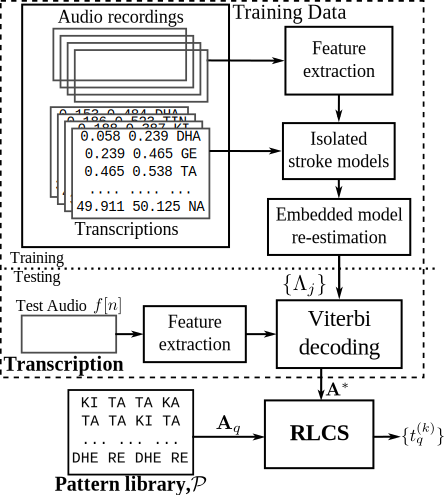
\includegraphics[width=\textwidth]{blockDiags/blockDiagTablaDiscovery.pdf}
\caption[Block diagram: Percussion pattern discovery in Indian art music]{A block diagram of percussion pattern discovery approach in Indian art music. The figure considers the example of \gls{tabla} solos for illustration.}
\label{fig:BD:tablaPattDiscovery}
\end{figure}

Using the simple definition of a pattern as a sequence of syllables, we use the scores of the compositions in the \acrshort{TSD} dataset (for \gls{tabla}) and \acrshort{UMSD} dataset (for mridangam) to generate all the $\pattLen$ length patterns that occur in the score collection. We sort them by their frequency of occurrence to get an ordered set of patterns for each stated length. We then manually choose musically representative patterns from this ordered set of most commonly occurring patterns to form a set of query patterns $\pattSet$. We create a set of query patterns of length $L = {4, 6, 8, 16}$. These lengths were chosen based on the structure of \glspl{tala} in the score collections (\gls{adi} and \gls{rupaka} \gls{tala} in mridangam solo dataset and \gls{teental} in \gls{tabla} solo dataset). 
\begin{table}
\centering
\begin{tabular}{@{}lp{8cm}cr@{}} \toprule
ID & \centering Pattern & $\pattLen$ & Count\tabularnewline \midrule
$\percPattSeq_1$ & \syl{DHE, RE, DHE, RE, KI, TA, TA, KI, NA, TA, TA, KI, TA, TA, KI, NA} & 16 & 47\tabularnewline \addlinespace[5pt]
$\percPattSeq_2$ & \syl{TA, TA, KI, TA, TA, KI, TA, TA, KI, TA, TA, KI, TA, TA, KI, TA} & 16 & 10\tabularnewline \addlinespace[5pt]
$\percPattSeq_3$ & \syl{TA, KI, TA, TA, KI, TA, TA, KI} & 8 & 61\tabularnewline \addlinespace[5pt]
$\percPattSeq_4$ & \syl{TA, TA, KI, TA, TA, KI} & 6 & 214\tabularnewline \addlinespace[5pt]
$\percPattSeq_5$ & \syl{TA, TA, KI, TA} & 4 & 379\tabularnewline \addlinespace[5pt]
$\percPattSeq_6$ & \syl{KI, TA, TA, KI} & 4 & 450\tabularnewline \addlinespace[5pt]
$\percPattSeq_7$ & \syl{TA, TA, KI, NA} & 4 & 167\tabularnewline \addlinespace[5pt]
$\percPattSeq_8$ & \syl{DHA, GE, TA, TA} & 4 & 97\tabularnewline \bottomrule
\end{tabular}
\caption[Query \gls{tabla} percussion patterns]{Query \gls{tabla} percussion patterns, their ID, length ($\pattLen$) and the number of instances in the \acrshort{TSD} dataset (Total instances: 1425). }\label{tab:pp:tablalib}
\end{table}

\tabref{tab:pp:tablalib} shows the query \gls{tabla} patterns used in this work obtained from the \acrshort{TSD} dataset. The table also shows their length and their count in the dataset, leading to a total of 1425 instances. We want a diverse collection of patterns to test if the algorithms generalize. Hence we choose patterns that have a varied set of syllables with different timbral characteristics, like syllables that are harmonic (\syl{DHA}), syllables played with a flam (\syl{DHE,RE}) and syllables having a bass component (\syl{GE}). 
\begin{table}
\centering
\begin{tabular}{@{}lp{8cm}cr@{}} \toprule
ID & \centering Pattern & $\pattLen$ & Count\tabularnewline \midrule
$\percPattSeq_1$ & \syl{DH3, TA, DH3, TA, TH, DH3, TH, TA} & 8 & 70 \tabularnewline \addlinespace[5pt]
$\percPattSeq_2$ & \syl{TA, DH3, TA, TH, DH3, TH, TA, TM} & 8 & 69 \tabularnewline \addlinespace[5pt]
$\percPattSeq_3$ & \syl{DH3, TA, DH3, TA, TH, DH3} & 6 & 89 \tabularnewline \addlinespace[5pt]
$\percPattSeq_4$ & \syl{DH3, TA, TH, DH3, TH, TA} & 6 & 70 \tabularnewline \addlinespace[5pt]
$\percPattSeq_5$ & \syl{TA, TH, DH3, TH, TA, TM} & 6 & 69 \tabularnewline \addlinespace[5pt]
$\percPattSeq_6$ & \syl{DH3, TA, TH, DH3} & 4 & 291 \tabularnewline \addlinespace[5pt]
$\percPattSeq_7$ & \syl{DH3, TA, DH3, TA} & 4 & 114 \tabularnewline \addlinespace[5pt]
$\percPattSeq_8$ & \syl{TH, DH3, TA, TH} & 4 & 102 \tabularnewline \addlinespace[5pt]
$\percPattSeq_9$ & \syl{TA, TH, DH3, TH} & 4 & 102 \tabularnewline \bottomrule
\end{tabular}
\caption[Query mridangam percussion patterns]{Query mridangam percussion patterns, their ID, length ($\pattLen$) and the number of instances in the \acrshort{UMSD} dataset (Total instances: 976). }\label{tab:pp:mridangamlib}
\end{table}

\tabref{tab:pp:mridangamlib} shows the query mridangam patterns used in this work obtained from the \acrshort{UMSD} dataset. The table also shows their length and their count in the dataset, leading to a total of 976 instances. As confirmed by a carnatic percussionist, these patterns are very commonly played in practice and hence are a good set of candidates to evaluate pattern discovery methodologies. 
%
\subsection{Automatic transcription}
%Given an audio recoding of percussion solo, automatic transcription refers to transcribing a given percussion solo audio recording into a time aligned sequence of syllables using syllable timbre models. 
An audio example of a percussion pattern is shown in \figref{fig:percpatt:tabla} for \gls{tabla}, and in \figref{fig:percpatt:mridangam} for mridangam. In the figures, we can see the pitched nature of some of the strokes, with clear onsets in many cases, but an overlap between adjacent strokes of the pattern. This needs a modeling of timbre, along with modeling of sequential information in syllables. 

Some \glspl{bol} of \gls{tabla} may be pronounced with a different vowel or consonant depending on the context, without altering the drum stroke \cite{chandola:98:ethno}. Furthermore, the \glspl{bol} and the strokes vary across different \glspl{gharana}, making the task of transcription of \gls{tabla} solos challenging. Mridangam syllables are further less specific as discussed earlier, and using the timbral grouping aims to address this challenge. To model the timbral dynamics of syllables, we build an \gls{HMM} for each syllable (analogous to a word-\gls{HMM}). We use these \glspl{HMM} along with a language model to transcribe an input audio solo recording into a sequence of syllables. 

The stereo audio is converted to mono, since there is no additional information in stereo channels. We use the \gls{MFCC} features to model the timbre of the syllables. To capture the temporal dynamics of syllables, we add the velocity and the acceleration coefficients of the \gls{MFCC}. The 13 dimensional  \gls{MFCC} features (including the zeroth coefficient) are computed from the audio with a frame size of 23.2 ms and a shift of 5.8 ms. We also explore the use of energy (as measured by the zeroth \gls{MFCC} coefficient) in transcription performance. Hence we have two sets of features, \acrshort{MFCCODA}, the 39 dimensional feature including the zeroth, delta and double-delta coefficients, and \acrshort{MFCCDA}, the 36 dimensional vector without the zeroth coefficient.
\begin{figure}
\centering
\includegraphics[width=\textwidth]{percPatterns/tabla-percpatt.pdf}
\caption[An example of a \gls{tabla} percussion pattern]{The waveform and spectrogram of an audio example of a \gls{tabla} percussion pattern shown with the onsets and the mapped syllable names from \tabref{tab:dataset:tsd}. The x-axis is time in seconds.}
\label{fig:percpatt:tabla}
\end{figure}
% 
\begin{figure}
\centering
\includegraphics[width=\textwidth]{percPatterns/mridangam-percpatt.pdf}
\caption[An example of a mridangam percussion pattern]{The waveform and spectrogram of an audio example of a mridangam percussion pattern shown with the onsets and the mapped syllable names from \tabref{tab:dataset:uks}. The x-axis is time in seconds.}
\label{fig:percpatt:mridangam}
\end{figure}

Using the features extracted from training audio recordings, we model each syllable $\sylSetVar_j$ using a 7-state left-to-right \gls{HMM} $\{\hmmSym_j\}$, $1 \leq j \leq \nSyllables$, including an entry and an exit non-emitting states. For \gls{tabla} solo transcription, $\nSyllables = 18$ while for mridangam solo transcription task, $\nSyllables = 21$. The emission density of each emitting state is modeled with a three component \gls{GMM} to capture the timbral variability in syllables. We experimented with higher number of components in the \glspl{GMM}, but with little performance improvement. 

The \acrshort{TSD} \gls{tabla} solo dataset is a parallel corpus of audio and time aligned syllabic transcriptions, each syllable \gls{HMM} is initialized through an isolated \gls{HMM} training of each syllable. The \acrshort{UMSD} mridangam solo dataset lacks such time aligned transcriptions and hence all syllables are initialized with a flat start \gls{HMM} using all the data in the dataset. Additionally for comparison, we report results with a flat start on \acrshort{TSD} \gls{tabla} dataset too. The initialized \glspl{HMM} are then trained further in an embedded model Baum-Welch re-estimation to get the final syllable \glspl{HMM}. 

Percussion solos in Indian art music are built hierarchically using short phrases, and hence some \glspl{bol}/\glspl{solkattu} tend to follow a \gls{bol}/\gls{solkattu} more often than others. In such a scenario, a language model\index{Language model} can improve transcription. In addition to a flat language model with uniform unigram and transition probabilities, i.e. $P(\sylVar_1 = \sylSetVar_j) = \nicefrac{1}{\nSyllables}$ and $P(\sylVar_{k+1} = \sylSetVar_j | \sylVar_{k} = \sylSetVar_i) = \nicefrac{1}{\nSyllables}$, with $1 \leq i,j \leq \nSyllables$ and $k$ being the sequence index, we explore the use of a bigram language model learned from data. The bigram language model is learned from all the scores in the training data. 

For testing, we treat the feature sequence extracted from test audio file to have been generated from a first order time-homogeneous discrete Markov chain, which can consist of any finite length sequence of syllables. From the extracted feature sequence, we use the \glspl{HMM} $\{\hmmSym_j\}$ and a syllable network constructed from the language model to do a Viterbi (forced) alignment\index{Viterbi decoding}, which provides the most likely sequence of syllables and their onset timestamps, given as $\percPattSeq^{\optstar} = [(\timeVar_1,\sylVar_1), (\timeVar_2,\sylVar_2), \cdots, (\timeVar_{\optstar},\sylVar_{\pattLen^{\optstar}})]$, where $\timeVar_i$ is the onset time of $\sylVar_i$ and $\pattLen^{\optstar}$ is the length of the transcribed sequence. Similar to the experiments with Beijing opera, all the transcription experiments were done using \gls{HTK}~\cite{young:06:htkbook}. 
%
\subsection{Approximate pattern search}
The automatically transcribed output syllable sequence $\percPattSeq^{\optstar}$ is used to search for the query patterns. Transcription is often inaccurate in both the sequence of syllables and in the exact onset times of the transcribed syllables. We need to handle both these errors in a pattern search task from audio. We primarily focus on the errors in syllabic transcription in this work. We use the syllable boundaries output by the Viterbi algorithm, without any additional post processing. We can improve the output syllable boundaries using an onset detector \cite{bello:05:onset}, but we leave this task to future work. 

Searching of a query syllable sequence in a transcribed sequence of syllables is akin to string search. As discussed in the case of \gls{jingju} percussion pattern transcription task, errors in transcription are mainly insertions (\strInsErr), deletions (\strDelErr), substitutions (\strSubErr), and transpositions (\strTrnErr). Further, the query pattern is to be searched in the whole transcribed composition, where several instances of the query can occur. With both these issues, the problem of pattern search can be addressed as a subsequence search. \acrfull{RLCS} method is a suitable choice for such a case. \gls{RLCS} is a subsequence search method that searches for roughly matched subsequences while retaining the local similarity \cite{lin:11:rlcs}. We make further enhancements to \gls{RLCS} to handle the \strInsErr, \strDelErr\ and \strSubErr\ errors in transcription. 

We use a modified version of the \gls{RLCS} approach as proposed by \citeA{lin:11:rlcs} with changes proposed by \citeA{dutta:14:rlcs} to handle substitution errors. We propose a further enhancement to handle insertions and deletions, and explore its use in the current task. \citeA{dutta:14:rlcs} used a modified version of \gls{RLCS} for motif spotting in \glspl{alapana} of Carnatic music. We propose to use a similar approach with minor modifications to suit the symbolic domain specific to our use case. We first present a general form of \gls{RLCS} and then discuss different variants of the algorithm.

Given a query pattern $\percPattSeq_q \in \pattSet$ of length $\pattLen_q$ and a reference sequence (transcribed syllable sequence) $\percPattSeq^{\optstar}$ of length $\pattLen_{\optstar}$, \gls{RLCS} uses a dynamic programming approach to compute a score matrix (of size $\pattLen_{\optstar} \times \pattLen_{q}$) between the reference and the query with a rough length of match. We can use a threshold on the score matrix to obtain the instances of the query occurring in the reference. We can then use the syllable boundaries in the output transcription and retrieve the audio segment corresponding to the match.

For the ease of notation, we index the transcribed syllable sequence $\percPattSeq^{\optstar}$ with $i$ and the query syllable sequence $\percPattSeq_q$ with $j$ in this section. We compute the rough and actual length of the subsequence matches similar to the way computed by \citeA{dutta:14:rlcs}. At every position $(i,j)$, a syllable is included into the matched subsequence if $d(\sylVar_i,\sylVar_j) \leq \sylDistThres$, where $d(\sylVar_i,\sylVar_j)$ is the timbral distance between the syllables at positions $i$ and $j$ in the transcription and query, respectively. $\sylDistThres$ is the threshold distance below which the two syllables are said to be equivalent. The matrices of rough length of match ($\rlcsLen$) and the actual length of match ($\rlcsLen^a$) are updated as,
\begin{eqnarray}
\rlcsLen(i,j) &=& \rlcsLen(i-1,j-1) + (1-d(\sylVar_i,\sylVar_j)) . \indicator_d \label{eq:rlcs:roughLength}\\
\rlcsLen^a(i,j) &=& \rlcsLen^a(i-1,j-1) + \indicator_d \label{eq:rlcs:trueLength}
\end{eqnarray}
where, $\indicator_d$ is an indicator function that takes a value of 1 if $d(\sylVar_i,\sylVar_j) \leq \sylDistThres$, else 0. The matrix $\rlcsLen$ thus contains the length of rough matches ending at all combinations of the syllable positions in reference and the query. The rough length and an appropriate distance measure handles the substitution errors during transcription. 

To penalize insertion and deletion errors, we compute a ``density'' of match using two measures called the \gls{WAR} and \gls{WAQ}, respectively. The \gls{WAR} ($\warMat$) and \gls{WAQ} ($\waqMat$) matrices are initialized to $\warMat_{i,j}=\waqMat_{i,j} = 0$ when $i.j = 0$, and propagated as,
\begin{equation}\label{eq:rlcs:war}
\warMat_{i,j} = 
\begin{cases}
\warMat_{i-1,j-1}+1 & d(\sylVar_i,\sylVar_j) \leq \sylDistThres\\
\warMat_{i-1,j}+1 & d(\sylVar_i,\sylVar_j) > \sylDistThres,\, \rlcsLen_{i-1,j} \geq \rlcsLen_{i,j-1}\\
\warMat_{i,j-1} & d(\sylVar_i,\sylVar_j) > \sylDistThres,\, \rlcsLen_{i-1,j} < \rlcsLen_{i,j-1}
\end{cases}
\end{equation}
%
\begin{equation}\label{eq:rlcs:waq}
\waqMat_{i,j}=
\begin{cases}
\waqMat_{i-1,j-1}+1 & d(\sylVar_i,\sylVar_j) \leq \sylDistThres\\
\waqMat_{i-1,j} & d(\sylVar_i,\sylVar_j) > \sylDistThres,\, \rlcsLen_{i-1,j}\geq \rlcsLen_{i,j-1}\\
\waqMat_{i,j-1}+1 & d(\sylVar_i,\sylVar_j) > \sylDistThres,\, \rlcsLen_{i-1,j} < \rlcsLen_{i,j-1}
\end{cases}
\end{equation}
Here, $\warMat_{i,j}$ is the length of substring containing the subsequence match ending at the $i^\mathrm{th}$ and the $j^\mathrm{th}$ position of the reference and the query, respectively. $\waqMat_{i,j}$ represents a similar measure in the query. When incremented, $\warMat_{i,j}$ and $\waqMat_{i,j}$ are incremented by 1 similar to the way formulated by \citeA{lin:11:rlcs}. At the same time, the increment is done based on the conditions formulated by \citeA{dutta:14:rlcs}.

Using the rough length of match ($\rlcsLen$), actual length of match ($\rlcsLen^a$), and width measures ($\warMat$ and $\waqMat$), we compute a score matrix $\rlcsWt$ that incorporates penalties for substitutions, insertions, deletions, and additionally, the fraction of the query matched as, 
\begin{equation}\label{eq:rlcs:score}
\rlcsWt_{i,j} = 
\begin{cases}
\begin{array}{ll}
\left[\rlcsMixParam\!\cdot\!\warpfn\!\left(\frac{\rlcsLen_{i,j}}{\warMat_{i,j}}\right) + (1-\rlcsMixParam)\!\cdot\!\warpfn\!\left(\frac{\rlcsLen_{i,j}}{\waqMat_{i,j}}\right)\right]\!\!\cdot\!\!\frac{\rlcsLen_{i,j}}{\pattLen_q} & \mathrm{if}\,\,\frac{\rlcsLen^{a}_{i,j}}{\pattLen_q}\!\!\geq\minFracThres\\ 0 & \mathrm{otherwise}
\end{array}\end{cases}
\end{equation}
where $\rlcsWt_{i,j}$ is the score for the match ending at the $i^\mathrm{th}$ and the $j^\mathrm{th}$ position of the reference and the query, respectively. $\warpfn$ is a warping function for the rough match length densities $\frac{\rlcsLen_{i,j}}{\warMat_{i,j}}$ in the reference and $\frac{\rlcsLen_{i,j}}{\waqMat_{i,j}}$ in the query. The parameter $\rlcsMixParam$ controls their weights in the convex combination for score computation. The term $\frac{\rlcsLen_{i,j}^{a}}{\pattLen_q}$ is the fraction of the query length matched and is used for thresholding the minimum fraction of the query to be matched. The parameter $\minFracThres$ is the threshold for the minimum fraction that contributes to the score. Starting with all combinations of $i$ and $j$ as the end points of the match in the reference and the query, respectively, we perform a traceback to get the starting points of the match.

\gls{RLCS} algorithm outputs a match when the score is more than a score threshold $\rlcsScoreThres$. However, with a simple score thresholding, we get multiple overlapping matches, from which we select the match with the highest score. If the scores of multiple overlapping matches are equal, we select the ones that have the lowest width (\gls{WAR}). This way, we obtain a match that has the highest score density. We use these non-overlapping matches and the corresponding syllable boundaries to retrieve the audio patterns.
%
\subsubsection{Variants of \gls{RLCS}}
The generalized \gls{RLCS} provides a robust framework for subsequence search. The parameters $\minFracThres$, $\rlcsMixParam$, $\rlcsScoreThres$ and $\sylDistThres$ can be tuned to make the algorithm more sensitive to different kinds of transcription errors. The variants we consider here use different distance measures $d(\sylVar_i,\sylVar_j)$ in \eqnref{eq:rlcs:roughLength} to handle substitutions and different functions $f(.)$ in \eqnref{eq:rlcs:score} to handle insertions and deletions. We explore these variants for the current task and evaluate their performance.

In a default \gls{RLCS} configuration (\rlcso), we only consider exact syllable matches. We set $\sylDistThres = 0$ and use a binary distance metric based on the syllable label, i.e. $d(\sylVar_i,\sylVar_j) = 0$ if $\sylVar_i = \sylVar_j$, and 1 otherwise. Further, an identity warping function, $\warpfn(u) = u$ is used. The rough length match densities can be transformed using a non-linear warping function to penalize low density values more than the higher ones, leading to another variant of \gls{RLCS} called the warped density \gls{RLCS} (denoted as \rlcss\ in this chapter). In this dissertation, we only explore warping functions of the form, 
\begin{equation}\label{eq:rlcs:warp}
\warpfn(u) = \frac{\mathrm{e}^{\warpParam u}-1}{\mathrm{e}^{\warpParam}-1}
\end{equation}
where $\warpParam > 0$ is a parameter to control warping, larger values of $\warpParam$ lead to more deviation from an identity transformation. \rlcso\ is a limiting case of \rlcss\ when $\warpParam \rightarrow 0$. 

We hypothesize that the substitution errors in transcription are due to the confusion between timbrally similar syllables. A timbral similarity (distance) measure between the syllables can thus be used to make an \gls{RLCS} algorithm robust to specific kinds of substitution errors. In essence, we want to disregard and give a greater allowance for substitutions between timbrally similar syllables during \gls{RLCS} matching. Computing timbral similarity is a wide area of research and has many different proposed methods \cite{pachet:04:similarity}, but we restrict ourselves to a basic timbral distance measure: the Mahalanobis distance between the cluster centers obtained using a k-means clustering of \gls{MFCC} features (with 3 clusters) from isolated audio examples of each syllable \cite{aucouturier:02:similarity}. We call this variant of \gls{RLCS} that uses a timbral distance $d(\sylVar_i,\sylVar_j)$ as \rlcsd\ and experiment with different thresholds $\sylDistThres$. % For better reproducibility of the work in this paper, an implementation of the different variants of \gls{RLCS} described is available\footnote{\url{http://compmusic.upf.edu/ismir-2015-tabla}}.
%
\subsection{Results and discussion}
Similar to the results in \secref{sec:boperc:results}, we present an evaluation of percussion pattern transcription and discovery for both \gls{tabla} and mridangam solo datasets. The results of automatic transcription and those of approximate pattern search are presented separately in each case. We first present it for the \gls{tabla} solo dataset (\acrshort{TSD} dataset), followed by the mridangam solo dataset (\acrshort{UMSD} dataset). It is important to note the contrast between the two datasets being evaluated: the recordings in \acrshort{UMSD} dataset have already been segmented into short phrases with the query patterns being the same order of length as the test audio recording, while the recordings in \acrshort{TSD} dataset are full length compositions spanning multiple \gls{taal} cycles, and hence much longer than the query patterns. We will also analyze the effect of this difference in datasets on the results of pattern search. 
% 
\subsubsection{Results on \gls{tabla} solo dataset}
The \gls{tabla} solo dataset (\acrshort{TSD} dataset) described in \secref{sec:tsdataset} is used to evaluate the performance of transcription and discovery in \gls{tabla} percussion solo recordings. The results of automatic transcription is first presented, and the best performing transcription system is used to present the results of approximate pattern search using different variants of \gls{RLCS}. 

The performance of automatic transcription is shown in \tabrefs{tab:pptransResER:tabla}{tab:pptransResIsoER:tabla} as the mean value over the whole dataset in a leave-one-piece out cross validation experiment. The performance measures are Correctness (\corrMeas) and Accuracy (\accuMeas) as defined in \eqnref{eqn:pp:straccu}. We experimented with the two different \gls{MFCC} features (\acrshort{MFCCDA} and \acrshort{MFCCODA}), two different initializations of \glspl{HMM} (an isolated training and a flat start, both followed by embedded reestimation training) and two language models (a flat model and a bigram learned from data). 

With the parallel time aligned transcriptions in the dataset, we experiment with both a flat initialization of syllables with an isolated training initialization of syllable \glspl{HMM}, followed by embedded training. The results with flat start initialization of \glspl{HMM} is shown in \tabref{tab:pptransResER:tabla} and the results for \glspl{HMM} initialized with isolated stroke examples are shown in \tabref{tab:pptransResIsoER:tabla}. In each table, the results are shown for both a flat (uniform) language model that assumes equal unigram and bigram probabilities, and for a bigram language model learned from training data. The tables also show both training accuracy (measured on training data) and test accuracy (measured on test data). In both tables, the best performing combination with highest test Accuracy is shown in bold. For test data performance, the values underlined in each column of the tables are statistically equivalent to the best result (in a paired-sample t-test at 5\% significance levels).
\begin{table}
\centering
\begin{tabular}{@{}clccccc@{}} \toprule
 &  & \multicolumn{2}{c}{Training} &  & \multicolumn{2}{c}{Test}\tabularnewline
LM & Feature & \corrMeas & \accuMeas &  & \corrMeas & \accuMeas \tabularnewline \midrule
\multirow{2}{*}{Flat} & \acrshort{MFCCDA} & 67.82  & 46.05  &  & \underline{64.21}  & 37.94 \tabularnewline
 & \acrshort{MFCCODA} & 70.63  & 51.78  &  & \underline{66.30}  & \underline{43.86}\tabularnewline \addlinespace[5pt]
\multirow{2}{*}{Bigram} & \acrshort{MFCCDA} & \textbf{68.50}  & \textbf{50.48}  &  & \underline{\textbf{65.33}}  & \underline{\textbf{44.10}}\tabularnewline
 & \acrshort{MFCCODA} & 69.33  & 46.72  &  & \underline{64.49}  & 39.48\tabularnewline \bottomrule
\end{tabular}
\caption[Automatic transcription results on \gls{tabla} solo dataset (Flat start \acrshort{HMM})]{Automatic transcription results on the \acrshort{TSD} dataset (\gls{tabla}) using \glspl{HMM} initialized with a flat start for each syllable. The table shows both training and test performance, for both a flat and a bigram language model, using the Correctness (\corrMeas) and Accuracy (\accuMeas) performance measures. The best performing combination with highest test Accuracy is shown in bold. For test data performance, the values underlined in each column are statistically equivalent to the best result. All values are in percentage.}\label{tab:pptransResER:tabla}
\end{table}
%
\begin{table}
\centering
\begin{tabular}{@{}clccccc@{}} \toprule
 &  & \multicolumn{2}{c}{Training} &  & \multicolumn{2}{c}{Test}\tabularnewline
LM & Feature & \corrMeas & \accuMeas &  & \corrMeas & \accuMeas \tabularnewline \midrule
\multirow{2}{*}{Flat} & \acrshort{MFCCDA} & 68.42  & 52.69  &  & 64.07  & 45.01\tabularnewline
 & \acrshort{MFCCODA} & 68.91  & 56.78  &  & 64.26  & 49.27\tabularnewline \addlinespace[5pt]
\multirow{2}{*}{Bigram} & \acrshort{MFCCDA} & 70.16  & 57.83  &  & \underline{65.53}  & 49.97\tabularnewline
 & \acrshort{MFCCODA} & \textbf{70.71}  & \textbf{60.77} &  & \underline{\textbf{66.23}}  & \underline{\textbf{53.13}}\tabularnewline \bottomrule
\end{tabular}
\protect\caption[Automatic transcription results on \gls{tabla} solo dataset (Isolated start \acrshort{HMM})]{Automatic transcription results on the \acrshort{TSD} dataset (\gls{tabla}) using \glspl{HMM} initialized using isolated stroke examples for each syllable.}\label{tab:pptransResIsoER:tabla}
\end{table}

Overall, we see a best test Accuracy of 53.13\% for isolated stroke initialization with the \acrshort{MFCCODA} feature and a bigram language model, which justifies the use of robust approximate string search algorithm for pattern retrieval. We see that the Accuracy measure for all cases is lower than the Correctness measure, which shows that there are a significant number of insertion errors in transcription. Training Accuracy is higher than test Accuracy, but with a small margin showing that there is some difficulty in modeling unseen data. Isolated stroke \gls{HMM} initialization improves performance, and hence it is useful to work with time aligned transcriptions. The use of a bigram language model learned from data improves the transcription performance when using isolated stroke \gls{HMM} initialization. With the features, when using isolated stroke \gls{HMM} initialization, we see that the use of the energy co-efficient in \acrshort{MFCCODA} performs better when compared to the feature \acrshort{MFCCDA}, which shows that the use of relative volume dynamics between strokes improves transcription performance. 
%
\begin{table}
\centering
\begin{tabular}{@{}lcccc@{}}
\toprule 
Variant & Parameter & Precision (\precision) & Recall (\recall) & f-measure (\fmeas) \tabularnewline \midrule
Baseline & - & 0.479 & 0.254 & 0.332 \tabularnewline \addlinespace[2pt]
\rlcso & $\sylDistThres=$ 0 & 0.384 & 0.395 & 0.389\tabularnewline \addlinespace[2pt]
\rlcsd & $\sylDistThres=$ 0.3 & 0.139 & 0.466 & 0.214\tabularnewline
\rlcsd & $\sylDistThres=$ 0.6 & 0.084 & 0.558 & 0.145\tabularnewline
\rlcss & $\warpParam=$ 1 & 0.412 & 0.350 & 0.378\tabularnewline
\rlcss & $\warpParam=$ 4 & 0.473 & 0.268 & 0.342\tabularnewline
\rlcss & $\warpParam=$ 7 & 0.482 & 0.259 & 0.336\tabularnewline
\rlcss & $\warpParam=$ 9 & 0.481 & 0.258 & 0.335\tabularnewline \bottomrule
\end{tabular}
\caption[Performance of approximate pattern search on \gls{tabla} solo dataset]{Performance of approximate pattern search on \acrshort{TSD} dataset (\gls{tabla}) using different \gls{RLCS} variants using the best performing parameter settings for \rlcso\ ($\minFracThres = 0.875$, $\rlcsMixParam = 0.76$ and $\rlcsScoreThres = 0.6$).}\label{tab:rlcsresults:tabla}
\end{table}

We use the output transcriptions from the best performing combination (\acrshort{MFCCODA} and a bigram language model) to report the performance of pattern search with approximate string matching in \tabref{tab:rlcsresults:tabla}, using different \gls{RLCS} variants for the query patterns from \tabref{tab:pp:tablalib}. For pattern retrieval, we don't evaluate the accuracy of boundary segmentation. However, we call a retrieved pattern from \gls{RLCS} as \textit{correctly retrieved} if it has at least a 70\% overlap with the pattern instance in ground truth. 

To evaluate pattern search performance, we use the standard information retrieval measures precision (\precision), recall (\recall) and their harmonic mean f-measure (\fmeas). To form a baseline for string search performance with the output transcriptions, we used an exact string search algorithm and report its performance in \tabref{tab:rlcsresults:tabla} (shown as Baseline). We see that the baseline has a precision that is similar to transcription performance, but a very poor recall leading to a poor f-measure. % To evaluate pattern search performance, we use the standard information retrieval measures precision (the ratio between the number of correctly retrieved patterns and all retrieved patterns) and recall (the ratio between number of correctly retrieved patterns and the patterns in the ground truth). The harmonic mean of precision and recall, the f-measure is also reported.

To establish the optimum parameter settings for \gls{RLCS}, we performed a grid search over the values of $\rlcsMixParam$, $\minFracThres$ and $\rlcsScoreThres$ with \rlcso. The parameters $\rlcsMixParam$ and $\rlcsScoreThres$ are varied in the range 0 to 1. To ensure that the minimum length of the pattern matched is at least 2, we varied $\minFracThres$ in the range, $\nicefrac{1.1}{\min(\pattLen_q)} < \minFracThres < 1$. The parameter $\rlcsMixParam$ is the convex sum parameter for the contribution of the rough match length density of the reference and the query towards the final score. With increasing $\rlcsMixParam$, we give more weight to the reference length ratio, allowing more insertions. We observed a poor true positive rate with larger $\rlcsMixParam$, and hence we validate the observation that insertion errors contribute to a majority of transcription errors. 

The best average f-measure over all the query patterns in an experiment using \rlcso\ is reported in \tabref{tab:rlcsresults:tabla}. We see that \rlcso\ improves the recall, but with a lower precision and an improved f-measure, showing that the flexibility in approximate matching provided by \gls{RLCS} comes at the cost of additional false positives. It is observed that the patterns composed of smaller repetitive patterns (and hence having ambiguous boundaries) result in a poor precision (e.g. $\percPattSeq_2$ and $\percPattSeq_3$ in \tabref{tab:pp:tablalib} with a precision of 0.108 and 0.239, respectively). Both are commonly played patterns with several repetitions and have a poor precision due to incorrect segmentation. $\percPattSeq_1$ in \tabref{tab:pp:tablalib}, on the contrary, has non-ambiguous boundaries leading to a good precision of 0.692. The effect of the length of a pattern on precision is also evident. Small patterns (with $\pattLen=4$) that have non-ambiguous boundaries (e.g. $\percPattSeq_8$ in \tabref{tab:pp:tablalib} with a precision of 0.384) have a poor precision as compared to longer patterns with non-ambiguous boundaries (e.g. $\percPattSeq_1$). The reason for this is that the smaller patterns are more prone to errors as the search algorithm has to match a lower number of syllables. 

The values of $\minFracThres$, $\rlcsMixParam$ and $\rlcsScoreThres$ that give the best f-measure with \rlcso\ are then fixed for all subsequent experiments to compare the performance of the proposed \gls{RLCS} variants. The results with other variants of \gls{RLCS} are also reported in \tabref{tab:rlcsresults:tabla}. The results from \rlcsd\ show that the use of a timbral syllable distance measure with higher threshold $\sylDistThres$ further improves the recall, but with a much lower precision and f-measure. Although we find matches that have substitution errors using the distance measure, we retrieve additional matches that do not have substitution errors contributing to additional false positives. On the contrary, using a non-linear warping function $f(.)$ in \rlcss\ improves the precision with larger values of $\warpParam$. The penalties on matches with higher number of insertions and deletions is large and they are left out, leading to a good precision at the cost of a poorer recall. We observe that both the above mentioned variants improve either precision or recall at the cost of the other measure. They need further exploration with better timbral similarity measures to be combined in an effective way to improve the search performance.
%
\subsubsection{Results on mridangam solo dataset}
Similar to an evaluation on the \gls{tabla} solo dataset, we present a parallel evaluation with the mridangam solo dataset (\acrshort{UMSD} dataset). Unlike the \gls{tabla} solo dataset, since the mridangam solo dataset does not have time aligned ground truth transcriptions, we report automatic transcription results only for flat start embedded \gls{HMM} training. With the best performing combination, we then report results of pattern search using different \gls{RLCS} variants using the query patterns from \tabref{tab:pp:mridangamlib}. We use identical definitions of performance measures as used while reporting results for \gls{tabla} solo dataset. 
% \comment{Mapping, HMM training, testing, basic results, inferences, ... expts. to be completed}
\begin{table}
\centering
\begin{tabular}{@{}clccccc@{}} \toprule
 &  & \multicolumn{2}{c}{Training} &  & \multicolumn{2}{c}{Test}\tabularnewline
LM & Feature & \corrMeas & \accuMeas &  & \corrMeas & \accuMeas\tabularnewline \midrule
\multirow{2}{*}{Flat} & \acrshort{MFCCDA} & 76.66  & 59.43  &  & \underline{74.08}  & 55.64\tabularnewline
 & \acrshort{MFCCODA} & \textbf{76.63}  & \textbf{63.79}  &  & \underline{\textbf{74.13}}  & \underline{\textbf{60.23}}\tabularnewline \addlinespace[5pt]
\multirow{2}{*}{Bigram} & \acrshort{MFCCDA} & 78.12  & 57.69  &  & 75.90  & 54.02\tabularnewline
 & \acrshort{MFCCODA} & 78.78  & 60.54  &  & 76.50  & 57.38\tabularnewline \bottomrule
\end{tabular}
\caption[Automatic transcription results on the mridangam solo dataset]{Automatic transcription results on the \acrshort{UMSD} dataset using \glspl{HMM} trained using a flat start for each syllable. The table shows both training and test performance, for both a flat and a bigram language model, using the Correctness (\corrMeas) and Accuracy (\accuMeas) performance measures. The best performing combination with highest test Accuracy is shown in bold. For test data performance, the values underlined in each column are statistically equivalent to the best result.}\label{tab:pptransRes:mridangam}
\end{table}

The results of automatic transcription are shown in \tabref{tab:pptransRes:mridangam} for all the combinations of conditions. For test data performance, the values underlined in each column of the table are statistically equivalent to the best result (in a paired-sample t-test at 5\% significance levels). Overall, we see a best test Accuracy of 60.23\% for \acrshort{MFCCODA}. Similar to results on \gls{tabla} dataset, we see that the Accuracy measure for all cases is lower than the Correctness measure, which shows that there are a significant number of insertion errors in transcription. Training Accuracy is higher than test Accuracy, but with a small margin showing that there is some difficulty in modeling unseen data. With the features, we see that the use of the energy co-efficient in \acrshort{MFCCODA} performs better when compared to the feature \acrshort{MFCCDA}, which shows that the use of relative volume dynamics between strokes improves transcription performance.

Contrary to results on \gls{tabla} dataset, the use of a bigram language model learned from data does not improve the transcription performance. The better performing combination uses a flat language model. We hypothesize that it is because there is much more variety in mridangam stroke playing in the dataset and a bigram language model learned from training data restricts the possibility of unseen stroke sequences adversely. It also hints towards the use of better language models that can incorporate longer contexts than a simplistic bigram language model. 
\begin{table}
\centering
\begin{tabular}{@{}lcccc@{}}
\toprule 
Variant & Parameter & Precision (\precision) & Recall (\recall) & f-measure (\fmeas) \tabularnewline \midrule
Baseline & - & 0.902 & 0.492 & 0.637\tabularnewline \addlinespace[2pt]
\rlcso-1 & $\sylDistThres=0$  & 0.902 & 0.492 & 0.637\tabularnewline 
\rlcso-2 & $\sylDistThres=0$  & 0.258 & 0.762 & 0.386\tabularnewline \bottomrule
\end{tabular}
\caption[Performance of approximate pattern search on mridangam solo dataset]{Performance of approximate pattern search for baseline and \rlcso. \rlcso-1 shows the best f-measure in the experiments, obtained with parameter settings $\minFracThres = 0.525$, $\rlcsMixParam = 0.51$ and $\rlcsScoreThres = 0.95$, while \rlcso-2 shows the best recall achieved, obtained with parameter settings $\minFracThres = 0.275$,	$\rlcsMixParam = 0.11$ and	$\rlcsScoreThres = 0.45$.}\label{tab:rlcsresults:mridangam}
\end{table}

Using the output transcriptions from the best performing combination (\acrshort{MFCCODA} and a flat language model), we report the performance of approximate string matching with \gls{RLCS} algorithm for the query patterns from \tabref{tab:pp:mridangamlib}. \tabref{tab:rlcsresults:mridangam} shows the average results of pattern search with the \acrshort{UMSD} dataset (mridangam) with the \rlcso\ algorithm, with an exact string search baseline also shown. We further establish the optimum parameter settings for \gls{RLCS} using a grid search similar to experiments with \gls{tabla} solo dataset. The numbers in the table show the results for the best performing parameter settings. Since \rlcsd\ and \rlcss\ algorithms did not show any improvement in f-measure for \gls{tabla} solos, only the results of \rlcso\ are reported for mridangam solos. 

The results in \tabref{tab:rlcsresults:mridangam} are significantly different compared to \tabref{tab:rlcsresults:tabla} and need further explanation. We see a higher baseline performance using exact string match with a good precision and a poorer recall, indicating an improved transcription accuracy with mridangam. The lowest recall of 0.348 is achieved for pattern $\percPattSeq_3$ in \tabref{tab:pp:mridangamlib}. Further, interestingly, the best performing f-measure with \rlcso\ (shown in the table as \rlcso-1) is equivalent to the baseline, giving an identical performance. On closer inspection, we see that this is achieved at a high score threshold of $\rlcsScoreThres = 0.95$. Such a high score threshold makes the \gls{RLCS} algorithm to be equivalent to exact search, penalizing any approximate length scores and looking for exact matches. However, the best recall (of 0.762) with \rlcso\ (shown in the table as \rlcso-2) is obtained for a lower score threshold of $\rlcsScoreThres = 0.45$, but with a significantly lower f-measure of 0.386 as shown in the table. In the case of the mridangam dataset, \gls{RLCS} does not show a significant advantage in improving f-measure. In addition, we see that the results on \acrshort{UMSD} dataset are insensitive to a wide range of values of $\minFracThres$ and	$\rlcsMixParam$. 

Both these interesting observations can be explained from the nature of the \acrshort{UMSD} dataset. The dataset consists of audio files that contain short segmented phrases, with query patterns being in the same order of length as the test audio files. In such a case, the computed rough match lengths and densities are not well defined, leading to the insensitivity of the mixing parameter ($\rlcsMixParam$) and the minimum fraction of match parameter $(\minFracThres$). In addition, an algorithm that considers rough lengths but uses a binary distance measure (such as \rlcso) would provide no significant advantage over an exact search. We can summarize that the present formulation of \rlcso\ algorithm is advantageous only when the query patterns are much shorter than the audio recordings in which these patterns are being queried. In addition, there is hence a need to explore improvements to pattern search in cases such as the mridangam dataset, where a query pattern is being searched over a large number of audio files that also contain short phrases. However, a more comprehensive experimentation on larger datasets with such characteristics would be necessary to confirm this claim. 
\section{Conclusions}
The chapter presented a detailed formulation of the task of percussion pattern discovery in music cultures syllabic percussion systems. The approaches utilized the overall timbres of percussion strokes (either from a single drum or from an ensemble) to define patterns. An evaluation on percussion datasets in \gls{jingju} and Indian art music datasets formally showed the possibility of such an approach, along with its advantages and current limitations. The goal of evaluations on percussion datasets of \gls{jingju}, \gls{tabla} and mridangam was to present a methodology for transcription and discovery/classification of percussion patterns in syllabic percussion systems. The work presented was preliminary and not comprehensive, with a significant scope for deeper study and improvement. However, the basic idea of using a musically meaningful representation system to define and describe patterns is valid and useful. Beijing opera provided a useful test case for percussion pattern classification, showing promising results. 

We mainly addressed the unexplored problem of a discovering syllabic percussion patterns in Indian drum (\gls{tabla} and mridangam) solo recordings. The presented formulation used a parallel corpus of audio recordings and syllabic scores to create a set of query patterns, that were searched in an automatically transcribed (into syllables) piece of audio. We used a simplistic definition of a pattern and explored \gls{RLCS} based subsequence search algorithm, using an \gls{HMM} based automatic transcription. Compared to a baseline, we showed that the use of approximate string search algorithms improved the recall at the cost of precision. Additionally, proposed variants evaluated on the \acrshort{TSD} dataset improved either the precision or recall, but do not provide a significant improvement in the f-measure over the basic \gls{RLCS}. Similar experiments on the \acrshort{UMSD} dataset showed a better transcription performance, while pointing out a limitation of the \gls{RLCS} approach when querying patterns in segmented short audio files. 

For future work, we aim to improve syllable boundaries output by transcription using onset detection. Inclusion of rhythmic information can be an interesting aspect in defining and discovering percussion patterns, and will help in evaluating the task of pattern discovery with a more inclusive definition of a percussion pattern. The next steps would be to incorporate better timbral similarity measures, include segment boundaries into the \gls{RLCS} algorithm formulation and effectively combine the proposed variants, while addressing its limitations when searching short audio files.
%
% Beijing Opera as a test case first - instrument recognition (ICASSP 2014)
%
% Percussion transcription is an important step towards describing these percussion patterns. For such a task, we first estimate the onsets of each of the percussion instruments, use this information in percussion transcription - which can be used for describing the meter and rhythmic progression of the piece, as well as describing percussion patterns that are important descriptors of the piece. It is with this goal that we explore instrument specific onset detection of Beijing Opera percussion and present this study.
% 
%\begin{table}[t]
%\centering
%\begin{tabular}{|p{2.5cm}|c|c|c|}
%\hline 
 %& Feature & Corr. & Accu.\tabularnewline
%\hline 
%\hline 
%\multirow{2}{*}{\parbox[t]{2cm}{Flat language model}} & MFCC\_D\_A & 64.07 & 45.01\tabularnewline
%\cline{2-4} 
 %& MFCC\_0\_D\_A & 64.26 & 49.27\tabularnewline
%\hline 
%\multirow{2}{*}{\parbox[t]{2.5cm}{Bigram language model}} & MFCC\_D\_A & \textbf{65.53} & 49.97\tabularnewline
%\cline{2-4} 
 %& MFCC\_0\_D\_A & \textbf{66.23} & \textbf{53.13}\tabularnewline
%\hline 
%\end{tabular}
%\protect\caption{Transcription results showing the Correctness (Corr.) and Accuracy (Accu.) measures (in percentage) for different features and language models. In each column, the values in bold are statistically equivalent to the best result (in a paired-sample t-test at 5\% significance levels).}
%\label{table:transcription}
%\end{table}
%
%
%
%
%\begin{table}[t]
%\centering
%\begin{tabular}{|p{2.5cm}|c|c|c|}
%\hline 
 %& Feature & Corr. & Accu.\tabularnewline
%\hline 
%\hline 
%\multirow{2}{*}{\parbox[t]{2cm}{Flat language model}} & MFCC\_D\_A & 64.07 & 45.01\tabularnewline
%\cline{2-4} 
 %& MFCC\_0\_D\_A & 64.26 & 49.27\tabularnewline
%\hline 
%\multirow{2}{*}{\parbox[t]{2.5cm}{Bigram language model}} & MFCC\_D\_A & \textbf{65.53} & 49.97\tabularnewline
%\cline{2-4} 
 %& MFCC\_0\_D\_A & \textbf{66.23} & \textbf{53.13}\tabularnewline
%\hline 
%\end{tabular}
%\protect\caption{Transcription results showing the Correctness (Corr.) and Accuracy (Accu.) measures (in percentage) for different features and language models. In each column, the values in bold are statistically equivalent to the best result (in a paired-sample t-test at 5\% significance levels).}
%\label{table:transcription}
%\end{table}
%
% The rough length ratios $f_{i,j}^{\warMat} = g\!\left(\frac{\rlcsLen_{i,j}}{\warMat_{i,j}}\right)$ and $f_{i,j}^{\waqMat} = g\!\left(\frac{\rlcsLen_{i,j}}{\waqMat_{i,j}}\right)$ are functions of the length of the rough match in the reference and the query, respectively with a suitable warping function $g(.)$. The parameter $\rlcsMixParam$ controls their weights in the convex combination for score computation. The term $\frac{\rlcsLen_{i,j}^{a}}{L_k}$ is the fraction of the query length matched. The parameter $\minFracThres$ is the threshold for the minimum fraction that contributes to the score. 
% Substitution
% The substitutions are taken care by the distance metric $\delta_{ij}$ using which the rough length of the match is calculated (\secref{subsubsec:roughtmatch}). 
% Insertions and deletions
%In \eqnref{eq:score}, $f_{i,j}^{\warMat}$ and $f_{i,j}^{\waqMat}$ represents the densities of the length of the rough match in the reference and the query, respectively and, thus, are measure for the number of insertions and deletions. $\rlcsMixParam$ is the weighting factor for them.
% fraction of the query matched
% Finally, we have the term $\frac{\rlcsLen_{i,j}^{a}}{L_k}$ which is the fraction of the query length matched, $L_k$ is the length of the query. $\minFracThres$ is the threshold for the minimum fraction that accounts for the score.